\documentclass{article}
\usepackage[utf8]{inputenc}
\usepackage{geometry}
\usepackage{datetime2}
\usepackage{xparse}
\usepackage{amsmath}
\usepackage{booktabs}
\usepackage{array}
\usepackage{hyperref}


 \geometry{
 a4paper,
 total={170mm,257mm},
 left=20mm,
 top=20mm,
 }

 
 \usepackage{graphicx}
 \usepackage{titling}

 \title{Review Paper : Artificial Intelligence Application in Engineering Design 
}
% \author{Muhammad Qomaruz Zaman}
\date{18 March 2025}
 
 \usepackage{fancyhdr}
\fancypagestyle{plain}{%  the preset of fancyhdr 
    \fancyhf{} % clear all header and footer fields
    \fancyfoot[R]{}
    \fancyfoot[L]{}
    \fancyhead[L]{
\includegraphics[width=2cm]{ITS_pojok.pdf}}
    \fancyhead[R]{ \DTMnow}
}
\makeatletter
\def\@maketitle{%
  \newpage
  \null
  \vskip 1em%
  \begin{center}%
  \let \footnote \thanks
    {\LARGE \@title \par}%
    \vskip 1em%
    %{\large \@date}%
  \end{center}%
  \par
  \vskip 1em}
\makeatother

\usepackage{lipsum}  
% \usepackage{cmbright} % Change the font by zee

\begin{document}

\maketitle


\noindent\begin{tabular}{l @{ : } l}
        Nama                &  Septian Feter Arifianto \\  
        NIM                 &  6022251072 \\  
        Teacher             &  Muhammad Qomaruz Zaman, S.T., M.T., Ph.D.\\
        Mata Kuliah         &  Kecerdasan Buatan Assigment 1 \\
\vspace{0,2cm}
        Class name          &  Kelas X\\
        Authors             & Yüksel, N., Börklü, H. R., Sezer, H. K., Canyurt, O. E. \\
        Years              & 2023 \\
        Judul               & Artificial Intelligence Applications In Engineering Design \\
        GitHub Link & \url{https://github.com/septianfeter-arifianto/feter-data.git}\\
\end{tabular}
\vspace{1cm}

Yüksel, Börklü, Sezer, and Canyurt (2023) provide a comprehensive review of how artificial intelligence (AI) has been used in engineering and product design from 2006 to 2021. They cover both classical techniques (expert systems, fuzzy logic, artificial neural networks, genetic algorithms) and modern approaches (machine learning, deep learning), organizing applications by design stages—inspiration, ideation/concept generation, evaluation, optimization, decision‑making, and modeling. After four screening rounds across Scopus and Web of Science, the authors include 184 studies (132 journal and 52 conference papers). Their trend analysis shows a clear move toward data‑driven methods and explainable AI (XAI) after 2015, with figures summarizing methods and topics over time. Strengths of the review include its wide scope, a practical phase‑based taxonomy, and a flowchart to aid method selection. However, the work would benefit from a PRISMA flow diagram, a formal quality appraisal of included studies, and empirical testing of the selection flowchart. Overall, it is a timely and useful synthesis for researchers and practitioners, with clear opportunities to improve methodological transparency and practical uptake. (Yüksel et al., 2023).


\section*{1. Resume from the journal}
\subsection*{a. paragraph summary}
This systematic review maps how artificial intelligence (AI) has transformed engineering and product design over the last fifteen years, spanning conceptual and embodiment stages from inspiration to modelling. The authors synthesize 184 publications (132 journals, 52 conferences) harvested via Scopus and Web of Science (2006–2021) and show a decisive shift from rule‑based “classical AI” (expert systems, fuzzy logic, neural networks, genetic algorithms) toward data‑driven approaches—especially machine learning and deep learning—since roughly 2014, propelled by big data and affordable compute. They classify applications by design stage (inspiration; idea/concept generation; evaluation; optimization/decision‑making; modelling and retrieval) and discuss how deep models (e.g., CNNs, GANs) now support creative ideation, generative design, topology/shape optimization, and 2D→3D modelling; while fuzzy logic and expert systems remain valuable for interpretable evaluation and decision support when knowledge is tacit and data scarce. Explainable AI (XAI) emerges as a cross‑cutting requirement as black‑box models penetrate safety‑critical domains. A practical two‑level AI‑method selection flowchart is proposed: if sufficient (or synthesizable) data exist, prefer data‑driven methods; otherwise use rule‑based systems or evolutionary search, with hybrids encouraged when single methods underperform. Reported benefits include faster iteration, reduced cost, broader search of design spaces, and more objective evaluation; limitations include dataset scarcity (especially labelled 3D), long training times, and generalization gaps across tasks. The review calls for integrating form, function, and behaviour in generative pipelines, curating robust open design datasets, advancing XAI for trust, and shortening data/compute bottlenecks—anticipating continued dominance of machine/deep learning in human‑AI co‑creation workflows

\subsection*{b. Purpose and scope}

\begin{itemize}
    \item To synthesize AI methods used in engineering/product design during 2006–2021 and classify them by design stages and technique families.
    \item To compare classical vs. modern AI, highlight trends, and identify future research directions.
    \item To provide a practical selection flowchart guiding designers to the “right AI” for a given problem.
\end{itemize}

\subsection*{C. Functional definitions and assumptions}

\begin{itemize}
    \item “AI” spans rule‑based and data‑driven techniques; design stages are grouped into inspiration, ideation, evaluation, optimization/decision, modelling.
    \item Scope limited to English articles indexed in Scopus and Web of Science, years 2006–2021; final dataset n=184 after four‑stage screening.
\end{itemize}

\section*{2. Method (how the review was conducted)}
Data sources and search strategy. The review searched Scopus and Web of Science, using comprehensive Boolean strings that combined terms for artificial intelligence methods (e.g., fuzzy logic, expert systems, genetic algorithms, neural networks, machine learning, deep learning) with engineering/product‑design terms. The full search expressions are reported in Table 1 of the article.

\begin{figure}[htbp]
    \centering
    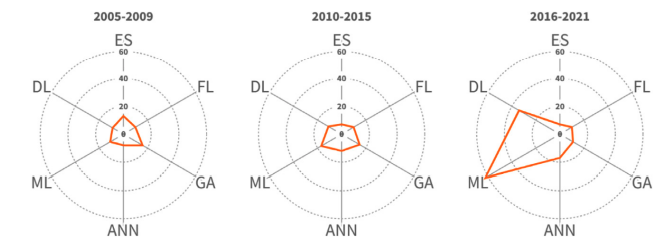
\includegraphics[width=0.9\linewidth]{Distribution of Paper.png}
    \caption{Distribution of publications involving the design based on AI methods between 2006 and 2021, (ES: Expert Systems, FL: Fuzzy Logic, GA: Genetic Algorithm, ANN: Artificial Neural Networks, ML: Machine Learning, DL: Deep Learning).}
    \label{fig:enter-label}
\end{figure}

\section*{3. Result}
\subsection*{a. Comparison with earlier reviews }
Earlier reviews typically focused either on classical AI in design (e.g., fuzzy/GA/ANN) or on modern data‑driven approaches in narrow subdomains (civil/construction, structural, AM). This paper’s novelty is its integrated perspective across both families, across all design stages, plus a selection flowchart, thus offering broader practical guidance than prior fragmented surveys.
\subsection*{b. Novelty}
\begin{itemize}
    \item A 15‑year panorama linking method families to specific design stages and demonstrating the post‑2014 surge of ML/DL in design.
    \item A two‑level AI selection algorithm (data‑availability first; then hybridization) for practitioners.
\end{itemize}
\subsection*{c. Analytic sensitivity }
rend conclusions are sensitive to database choice (Scopus/WoS), English‑only filter, and 2006–2021 window; expanding sources, languages, or years could alter counts and trend inflections.
\subsection*{d. Analytic scene }
Demonstrations span inspiration/ideation (semantic nets, social media mining, GAN‑based bionic design), evaluation (fuzzy/AHP; ML for creativity/affect), optimization (GA/PSO/DE; DL‑assisted topology), and modelling (2D→3D via VAE/GAN).

\section*{4. Limitations and potential biases}
\begin{itemize}
    \item Screening granularity (heavy reliance on abstracts before full sections).
    \item No quantitative meta‑analysis; conclusions are narrative/trend‑based.
    \item Temporal cutoff (2021) means very recent advances may be underrepresented
\end{itemize}

\section*{5. Implication}
Design practice: Use the flowchart—if data exist (or can be generated), prefer ML/DL; where explainability matters or data are scarce, lean on fuzzy/expert systems or evolutionary search, or hybrids and Org capability: Invest in data pipelines, compute, and XAI to embed trustworthy AI into early‑stage design.

\section*{6. Conclusion}
This is a useful, practitioner‑oriented survey: it goes beyond cataloguing to give actionable selection logic and a clear view of where AI adds the most value along the design pipeline. Its emphasis on data availability, hybridization, and explainability aligns well with real‑world constraints. The main caveat is the time window and source/language filters—for a living field like AI‑in‑design, periodic updates and broader indexing would further strengthen the guidance. Overall, I see it as a solid starting blueprint for teams planning an AI‑enabled design stack in 2026.






\end{document}
